\documentclass[notitlepage,showpacs,preprintnumbers,amsmath,amssymb,superscriptaddress,prd,onecolumn]{revtex4-1}
\pdfoutput=1
\usepackage{amsmath}
\usepackage[T1]{fontenc}
\usepackage{bm}
\usepackage{todonotes}
\usepackage[normalem]{ulem}
\usepackage{hyperref}
% \usepackage{showkeys}

\newcommand{\red}[1]{{\color{red} #1}}

\newcommand{\Neff}{\ensuremath{N_{\rm eff}}}
\newcommand{\DNeff}{\ensuremath{\Delta N_{\rm eff}}}
\newcommand{\dmsq}[1]{\ensuremath{\Delta m^2_{#1}}}
\newcommand{\uasq}[1]{\ensuremath{|U_{#1 4}|^2}}
\newcommand{\e}[1]{\ensuremath{\times10^{#1}}}

\newcommand{\fortepiano}{\texttt{FortEPiaNO}}
\newcommand{\dlsoda}{\texttt{DLSODA}}

\begin{document}
\title{\boldmath \fortepiano\ technical notes}

\author{S.\ Gariazzo}
\email{gariazzo@ific.uv.es}
\affiliation{Instituto de F{\'\i}sica Corpuscular  (CSIC-Universitat de Val{\`e}ncia), Valencia, Spain}

\author{P.F.\ de Salas}
\email{pablo.fernandez@fysik.su.se}
\affiliation{The Oskar Klein Centre for Cosmoparticle Physics,
Department of Physics, Stockholm University, SE-106 91 Stockholm, Sweden}

\author{S.\ Pastor}
\email{pastor@ific.uv.es}
\affiliation{Instituto de F{\'\i}sica Corpuscular  (CSIC-Universitat de Val{\`e}ncia), Valencia, Spain}


\maketitle


We present here the main features of
our code, \texttt{FORTran-Evolved PrimordIAl Neutrino Oscillations}
(\fortepiano) \cite{Gariazzo:2019gyi}.
The code is publicly available at the url
\url{https://bitbucket.org/ahep_cosmo/fortepiano_public}.


\section{Equations}
\fortepiano\ can compute oscillations with up to six neutrinos in the early universe.
Neutrinos, including the sterile ones, are always treated as ultra-relativistic particles, which is a good approximation if the
neutrino masses do not exceed $\mathcal{O}(\mbox{a few keV})$,
i.e.\ neutrinos are still fully relativistic at decoupling.
For larger masses, neutrinos may start to become non-relativistic before decoupling,
and in that case one should take into account the effect of the mass.

The code computes the evolution of the
$N\times N$ neutrino density matrix
\cite{deSalas:2016ztq,Mirizzi:2012we,Saviano:2013ktj,Mangano:2001iu}
\begin{equation}\label{eq:varrho-B4}
\varrho(x, y)
=
\left(
\begin{array}{ccccc}
\varrho_{ee}&\varrho_{e\mu}&\varrho_{e\tau}&\varrho_{es_1}&\ldots\\
\varrho_{\mu e}&\varrho_{\mu\mu}&\varrho_{\mu\tau}&\varrho_{\mu s_1}&\\
\varrho_{\tau e}&\varrho_{\tau\mu}&\varrho_{\tau\tau}&\varrho_{\tau s_1}&\\
\varrho_{s_1e}&\varrho_{s_1\mu}&\varrho_{s_1\tau}&\varrho_{s_1s_1}&\\
\vdots&&&&\ddots
\end{array}
\right)\,,
\end{equation}
which is the same for neutrinos and antineutrinos,
in terms of the comoving coordinates
$x\equiv m_e\, a$, $y\equiv p\, a$, $z\equiv T_\gamma\, a$ and $w\equiv T_\nu\,a$.
The momentum dependence of the density matrix $\varrho$ is taken into account
using a discrete grid of momenta, as described in section~\ref{ssec:momenta}.

When using $N$ neutrinos,
the mixing matrix is defined as
%
\begin{equation}\label{eq:mixing_matrix_nxn}
U=R^{(N-1)N} \ldots R^{1N}
R^{(N-2)(N-1)}\ldots R^{1(N-1)}
\ldots
R^{34} R^{24} R^{14} R^{23} R^{13} R^{12},
\end{equation}
%
following and extending the convention presented in Eq.~(12) of \cite{Gariazzo:2015rra},
where each $R^{ij}$ is a real rotation matrix described by the angle $\theta_{ij}$,
containing $\cos\theta_{ij}$ in the diagonal elements $ii$ and $jj$,
1 in the remaining diagonal elements,
$\sin\theta_{ij}$ ($-\sin\theta_{ij}$) in the off-diagonal element $ij$ ($ji$)
and zero otherwise:
\begin{equation}
\label{eq:rotationmatrix}
[R^{ij}]_{rs}=
\delta_{rs}
+
(\cos\theta_{ij}-1)(\delta_{ri}\delta_{si}+\delta_{rj}\delta_{sj})
+
\sin\theta_{ij}(\delta_{ri}\delta_{sj}-\delta_{rj}\delta_{si})\,.
\end{equation}
It enters the calculation of the rotated mass matrix
$\mathbb{M}_{\rm F}=U\mathbb{M}U^\dagger$,
where the diagonal mass matrix is
$\mathbb{M}=\text{diag}(m_1^2,\ldots,m_N^2)$.
Other matrices that we need to define are
%
\begin{equation}\label{eq:matterpotentials_nxn}
\mathbb{E}_\ell=\text{diag}(\rho_e, \rho_\mu, 0, \ldots)\,,
\qquad
\mathbb{P}_\ell=\text{diag}(P_e, P_\mu, 0, \ldots)\,,
\qquad
\mathbb{E}_\nu=S_a\frac{1}{\pi^2}\left(\int \mathrm{d}y y^3\varrho\right) S_a\,
\quad\mbox{with }S_a=\text{diag}(1,1,1,0,\ldots)\,,
\end{equation}
while the interaction matrices used in the the collision terms,
presented in section~\ref{sec:collint}, are
\begin{equation}
G^L=\text{diag}(g_L, \tilde g_L, \tilde g_L, 0,\ldots)\,,
\qquad
G^R=\text{diag}(g_R, g_R, g_R, 0,\ldots)\,,
\end{equation}
%
where $g_L=\sin^2\theta_W+1/2$, $\tilde g_L=\sin^2\theta_W - 1/2$, $g_R=\sin^2\theta_W$,
and $\theta_W$ is the weak mixing angle.
It is easy to see from the definitions of Eqs.~\eqref{eq:F_ab_sc} and \eqref{eq:F_ab_ann}
that the collision terms vanish when considering the interactions corresponding
only to sterile neutrinos.
When more than one sterile neutrino is considered, the damping terms between the different sterile neutrinos are therefore set to zero.

The definitions of comoving energy density and pressure,
which can be combined to obtain the comoving entropy density,
are written as:
\begin{eqnarray}
\rho_i
&=&
g_i
\int\frac{dp}{2\pi^2}\,
p^2 E_p \frac{1}{e^{E_p/z}\pm1}
\,,
\\
P
&=&
g_i
\int\frac{dp}{2\pi^2}\,
\frac{p^4}{3 E_p} \frac{1}{e^{E_p/z}\pm1}
\,,
\\
s
&=&
\frac{\rho+P}{z}
\,,
\end{eqnarray}
where the + (-) applies for fermions (bosons),
$i$ denotes the species, which has $g_i$ degrees of freedoms,
$p$ is the comoving momentum,
$E_p=\sqrt{p^2 + m_i^2}$, being $m_i$ the comoving mass of the particle,
and $z$ must be substituted with $w$ in the case of neutrinos.

To take into account finite temperature QED (FTQED) corrections
\cite{Fornengo:1997wa,Mangano:2001iu,Bennett:2019ewm},
we have to modify the total pressure and energy density of the fluid:
\begin{eqnarray}
P
&=&
\sum_{i=\gamma,{\nu_i},e,\mu}P_i
+
\delta P(x,z)
\,,\\
\rho
&=&
\sum_{i=\gamma,{\nu_i},e,\mu}\rho_i
+
\delta\rho(x,z)
\,,
\end{eqnarray}
where $\delta P$ and $\delta\rho$ are contributions that can be computed using FTQED.
It is convenient to define them
in terms of the following functions:
\begin{eqnarray}
J_a(r)
&=&
\frac{1}{\pi^2}
\int_0^\infty {\rm d}u \, u^a
\frac{\exp(\sqrt{u^2+r^2})}{\Big[\exp(\sqrt{u^2+r^2})+1\Big]^2}
\label{eq:j}
\,,\\
K_a(r)
&=&
\frac{1}{\pi^2}
\int_0^\infty {\rm d}u \, 
\frac{u^a}{\sqrt{u^2+r^2}}\,
\frac{1}{\exp(\sqrt{u^2+r^2})+1}
\label{eq:k}\,.
\end{eqnarray}
Let us also define for convenience:
\begin{eqnarray}
\mathcal{N}_p
&=&
\frac{2}{e^{E_p/z}+1}
\,,\\
\partial_x\mathcal{N}_p
&=&
-\frac{x\,e^{E_p/z}\,\mathcal{N}_p^2}{2z\,E_p}
\,,\\
\partial_z\mathcal{N}_p
&=&
\frac{
 e^{E_p/z}\,
 E_p\,
 \mathcal{N}_p^2
}{2 z^2}
\,,\\
\partial_x\partial_z\mathcal{N}_p
&=&
\frac{
 x\,
 e^{E_p/z}\,
 \mathcal{N}_p^2
}{2z^3}
\left(
 1
 -e^{E_p/z}\,\mathcal{N}_p
 +\frac{z}{E_p}
\right)
\,.
\end{eqnarray}
The contributions $\delta P$ and $\delta\rho$ can be expanded as a series of powers of the electron charge
$e^2=4\pi\alpha$, where $\alpha$ is the fine structure constant.
Taking into account the first orders of the expansion, and using $r=x/z$, for the pressure one has \cite{Bennett:2019ewm}
%
\begin{eqnarray}
\delta P(x,z)
&=&
\delta P^{(2)}(x/z)
+
\delta P^{(2+\ln)}(x,z)
+
\delta P^{(3)}(x/z)
+\ldots
\,,
\\
\delta P^{(2)}(r)
&=&
-
e^2 z^4\,K_2
\left(
 \frac{1}{6}
 +\frac{K_2}{2}
\right)
\,,\\
\delta P^{(2+\ln)}(x,z)
&=&
\frac{e^2 x^2}{16\pi^4}
\int\!\!\!\int_0^\infty
{\rm d}y\,
{\rm d}k\,
\frac{y\,k}{E_y E_k}
\ln
\left|
\frac{y+k}{y-k}
\right|
\mathcal{N}_y\,
\mathcal{N}_k
\,,\\
\delta P^{(3)}(r)
&=&
\frac{2e^3z^4}{3\pi}
\left(
K_2
+
\frac{r^2}{2} K_0
\right)^{3/2}
\,,
\end{eqnarray}
while for the energy density the various terms are
\begin{eqnarray}
\delta\rho(x,z)
&=&
\delta\rho^{(2)}(x/z)
+
\delta\rho^{(2+\ln)}(x,z)
+
\delta\rho^{(3)}(x/z)
+\ldots
\,,
\\
\delta\rho^{(2)}(r)
&=&
e^2 z^4
\left(
\frac{K_2^2}{2}
-\frac{K_2+J_2}{6}
-K_2 J_2
\right)
\,,\\
\delta\rho^{(2+\ln)}(x,z)
&=&
\frac{e^2 x^2}{16\pi^4}
\int\!\!\!\int_0^\infty
{\rm d}y\,
{\rm d}k\,
\frac{y\,k}{E_y E_k}
\ln
\left|
\frac{y+k}{y-k}
\right|
\mathcal{N}_y
\Big(
2z \partial_z \mathcal{N}_k
- \mathcal{N}_k
\Big)
\,,\\
\delta\rho^{(3)}(r)
&=&
\frac{e^3z^4}{\pi}
\left(
K_2
+
\frac{r^2}{2} K_0
\right)^{1/2}
\left(
J_2
+
\frac{r^2}{2} J_0
\right)
\,.
\end{eqnarray}

In order to compute the evolution of the neutrino density matrix \eqref{eq:varrho-B4},
we have to compute both the derivative of $\varrho$ (as a function of the momentum)
and of the comoving photon temperature $z$
with respect to our time parameter $x$.
The differential equations which the code solves are the following
\cite{deSalas:2016ztq,Mirizzi:2012we,Saviano:2013ktj,Mangano:2001iu}:
%
\begin{eqnarray}\label{eq:drho_dx_nxn}
\frac{{\rm d}\varrho(y)}{{\rm d}x}
&=&
\sqrt{\frac{3 m^2_{\rm Pl}}{8\pi\rho}}
\left\{
    -i \frac{x^2}{m_e^3}
    \left[
        \frac{\mathbb{M}_{\rm F}}{2y}
        -
        \frac{2\sqrt{2}G_{\rm F} y m_e^6}{x^6}
        \left(
            \frac{\mathbb{E}_\ell+\mathbb{P}_\ell}{m_W^2}
            +
            \frac{4}{3}\,\frac{\mathbb{E}_\nu}{m_Z^2}
        \right),
    \varrho
    \right]
    +\frac{m_e^3}{x^4}\mathcal{I(\varrho)}
\right\}\,,
\nonumber\\
\label{eq:dz_dx_nxn}
\frac{\mathrm{d}z}{\mathrm{d}x}
&=&
\cfrac{
{\displaystyle \sum_{\ell=e,\mu}}
\left[
\cfrac{r_\ell^2}{r} J_2(r_\ell)
\right]
+ G_1(r)
- \cfrac{1}{2\pi^2z^3}
    {\displaystyle \int_0^\infty \mathrm{d}y\,y^3\sum_{\alpha=e}^{s_{N_s}^{}}\cfrac{\mathrm{d}\varrho_{\alpha \alpha}}{\mathrm{d}x}}
}{
{\displaystyle \sum_{\ell=e,\mu}}
\Big[
r^2_\ell J_2(r_\ell)
+ J_4(r_\ell)
\Big]
+ G_2(r)
+ \cfrac{2\pi^2}{15}
}\,,
\end{eqnarray}
where $r_\ell=m_\ell/m_e\,r$.
The expressions for the $G_1$ and $G_2$ functions,
which again take into account the FTQED corrections, are written as
\cite{Mangano:2001iu,Bennett:2019ewm}:
%
\begin{eqnarray}
G_{1,2}(x,z)
&=&
G_{1,2}^{(2)}(x/z)
+
G_{1,2}^{(2+\ln)}(x,z)
+
G_{1,2}^{(3)}(x/z)
+
\ldots
\,,
\end{eqnarray}
%
\begin{eqnarray}
G_a(r)
&=&
\frac{K_2'}{6}
-K_2K_2'
+\frac{J_2'}{6}
+K_2'J_2
+K_2J_2'
\,,\\
G_1^{(2)}(r)
&=&
2\pi\alpha
\left[
  \frac{1}{r}
  \left(
    \frac{K_2}{3}
    + 2 K_2^2
    -\frac{J_2}{6}
    -K_2J_2
  \right)
  +
  G_a
\right]
\label{eq:g1}
\,,\\
G_2^{(2)}(r)
&=&
-8\pi\alpha
\left(
  \frac{K_2}{6}
  +\frac{J_2}{6}
  -\frac{1}{2}K_2^2
  +K_2J_2
\right)
+
2\pi\alpha r
G_a
\label{eq:g2}
\,,
\end{eqnarray}
%
\begin{eqnarray}
G_1^{(2+\ln)}(x,z)
&=&
\frac{e^2 x}{16\pi^4 z^3}
\int\!\!\!\int_0^\infty
{\rm d}y\,
{\rm d}k\,
\frac{y\,k}{E_y E_k}
\ln\left|\frac{y+k}{y-k}\right|
\Bigg\{
-x\bigg[
  z\Big(
    \partial_x\mathcal{N}_y\partial_z\mathcal{N}_k
    +
    \mathcal{N}_y\partial_x\partial_z\mathcal{N}_k
  \Big)
  -\mathcal{N}_y\partial_x\mathcal{N}_k
\bigg]
\nonumber\\
&&
\qquad\qquad\qquad\qquad
-\mathcal{N}_y\mathcal{N}_k
-z\mathcal{N}_y\partial_z\mathcal{N}_k
+\frac{x^2 (E_y^2+E_k^2)}{2 E_y^2 E_k^2}
\Big(
2z \mathcal{N}_y\partial_z \mathcal{N}_k
-\mathcal{N}_y \mathcal{N}_k
\Big)
\Bigg\}
\,,\\
G_2^{(2+\ln)}(x,z)
&=&
\frac{e^2 x^2}{16\pi^4 z^2}
\int\!\!\!\int_0^\infty
{\rm d}y\,
{\rm d}k\,
\frac{y\,k}{E_y E_k}
\ln\left|\frac{y+k}{y-k}\right|
\partial_z
\Big(
\mathcal{N}_y
\partial_z
\mathcal{N}_k
\Big)
\,,
\end{eqnarray}
%
\begin{eqnarray}
G_b(r)
&=&
\sqrt{K_2 + r^2 \frac{K_0}{2}}
\,,\\
G_c(r)
&=&
\frac{2J_2 + r^2 J_0}{2\Big(2K_2 + r^2 K_0\Big)}
\,,\\
G_1^{(3)}(r)
&=&
\frac{e^3}{4\pi} G_b
\left\{
 \frac{1}{r}\Big(2J_2-4K_2\Big)
 -2J_2'
 -r^2J_0'
 -r\Big(2K_0+J_0\Big)
 -G_c\Big[r(K_0-J_0)+K_2'\Big]
\right\}
\,,\\
G_2^{(3)}(r)
&=&
\frac{e^3}{4\pi} G_b
\left[
 G_c \Big(2J_2 + r^2 J_0\Big)
 -\frac{2}{r}J_4'
 -r\Big(3J_2'+r^2J_0'\Big)
\right]
\,,
\label{eq:g3}
\end{eqnarray}
%
where the prime denotes derivative with respect to $r$ and we dropped the explicit dependence on $r$ in the expressions for the $G$ functions.
For the sake of computational speed, we calculate and store lists for all the terms of Eq.~\eqref{eq:dz_dx_nxn}
which do not depend on the neutrino density matrix 
at the initialisation stage, and compute their values through interpolation during the real calculation.
The same happens for the energy densities of charged leptons, for which performing an interpolation
is much faster than computing an integral.
The interpolation, however, can be disabled during compilation (see the \texttt{README}),
with a $\lesssim20$\% increase of the running time.

In order to estimate the effective comoving neutrino temperature $w$, which is
not needed for the calculation but useful to understand the final results,
we use an equation similar to Eq.~\eqref{eq:dz_dx_nxn},
but considering only relativistic electrons, i.e.\ fixing $r_e=0$ in the equation.

The finite-temperature electromagnetic corrections are also taken into account in the calculation
of the electron mass, used in the collision terms.
The contribution to the electron mass, in comoving coordinates, is obtained as \cite{Fornengo:1997wa,Mangano:2001iu,Bennett:2019ewm}:
\begin{equation}
\delta m_e^2(x, y, z)
=
\frac{2\pi\alpha z^2}{3}
+
\frac{4\alpha}{\pi}
\int_0^\infty{\rm d}k\,
\frac{k^2}{E_k}
\frac{1}{e^{E_k/z}+1}
-
\frac{x^2\alpha}{\pi y}
\int_0^\infty{\rm d}k\,
\frac{k}{E_k}
\log\left|\frac{y+k}{y-k}\right|
\mathcal{N}_k
\,,
\end{equation}
so that the comoving electron mass must be replaced using $x^2\rightarrow x^2+\delta m_e^2$.
In the calculation of the collision integrals we ignore the log term that depends on $y$.

Finally, the effective number of degrees of freedom that the code returns in output is defined as:
\begin{eqnarray}
\Neff^e
&=&
\frac{8}{7}
\frac{\sum_i \rho_{\nu_i}}{\rho_\gamma}
\qquad\text{at early times,}
\\
\Neff^l
&=&
\frac{8}{7}
\left(\frac{11}{4}\right)^{4/3}
\frac{\sum_i \rho_{\nu_i}}{\rho_\gamma}
\qquad\text{at late times,}
\end{eqnarray}
being $\rho_\gamma$ the comoving energy density of photons and
$\rho_{\nu_i}$ the one of the $i$-th neutrino.


\section{Collision integrals}
\label{sec:collint}
The full collision terms are defined by the sum
of the contributions from neutrino--electron/positron scattering and
$e^\pm$ annihilation into neutrinos.
We neglect other reactions, such as $\mu^\pm$ annihilation (which only affects at very early temperatures when everything is in equilibrium)
and neutrino--neutrino scattering.
We therefore have \cite{deSalas:2016ztq}
%
\begin{eqnarray}
\mathcal{I}[\varrho(y)]
&=&
\frac{G_F^2}{(2\pi)^3y^2}
\left(\mathcal{I}_{\rm sc}^u + \mathcal{I}_{\rm ann}^u\right)\,,
\label{eq:collint}
\\
\mathcal{I}_{\rm sc} ^u
&=&
\int {\rm d}y_2 {\rm d}y_3 \frac{y_2}{E_2} \frac{y_4}{E_4}
\label{eq:I_sc}
\\
&&
\left\{\left(\Pi_2^s(y, y_4)+\Pi_2^s(y, y_2)\right)
    \left[
    F_{\rm sc}^{LL}\left(\varrho^{(1)}, f_e^{(2)}, \varrho^{(3)}, f_e^{(4)}\right)
    +F_{\rm sc}^{RR}\left(\varrho^{(1)}, f_e^{(2)}, \varrho^{(3)}, f_e^{(4)}\right)\right]\right.
    \nonumber\\
    &&\left.-2(x^2+\delta m_e^2)\Pi_1^s(y,y_3)
    \left[
     F_{\rm sc}^{RL}\left(\varrho^{(1)}, f_e^{(2)}, \varrho^{(3)}, f_e^{(4)}\right)
    +F_{\rm sc}^{LR}\left(\varrho^{(1)}, f_e^{(2)}, \varrho^{(3)}, f_e^{(4)}\right)
    \right]\nonumber
\right\}\,,
\\
\mathcal{I}_{\rm ann}^u
&=&
\int {\rm d}y_2 {\rm d}y_4 \frac{y_3}{E_3} \frac{y_4}{E_4}
\label{eq:I_ann}\\
    &&\left\{\Pi_2^a(y, y_4)F_{\rm ann}^{LL}\left(\varrho^{(1)}, \varrho^{(2)}, f_e^{(3)}, f_e^{(4)}\right)
    +\Pi_2^a(y, y_3)F_{\rm ann}^{RR}\left(\varrho^{(1)}, \varrho^{(2)}, f_e^{(3)}, f_e^{(4)}\right)\right.
\nonumber\\
    &&\left.+ (x^2+\delta m_e^2)\Pi_1^a(y,y_2)
    \left[
    F_{\rm ann}^{RL}\left(\varrho^{(1)}, \varrho^{(2)}, f_e^{(3)}, f_e^{(4)}\right)
    +F_{\rm ann}^{LR}\left(\varrho^{(1)}, \varrho^{(2)}, f_e^{(3)}, f_{e^+}^{(4)}\right)
    \right]\nonumber
\right\}\,,
\end{eqnarray}
where $E^2_i = \sqrt{x^2+y_i^2+\delta m_e^2}$ and
\begin{eqnarray}
\Pi_1^s(y,y_3)
&=&
y\,y_3\,D_1+D_2(y,y_3,y_2,y_4),
\\
\Pi_1^a(y,y_2)
&=&
y\,y_2\,D_1-D_2(y,y_2,y_3,y_4),
\\
\Pi_2^s(y,y_2)/2
&=&
y\,E_2\,y_3\,E_4\,D_1 + D_3 - y\,E_2 D_2(y_3,y_4,y,y_2) - y_3\,E_4 D_2(y,y_2,y_3,y_4),
\\
\Pi_2^s(y,y_4)/2
&=&
y\,E_2\,y_3\,E_4\,D_1 + D_3 + E_2\,y_3 D_2(y,y_4,y_2,y_3) + y\,E_4 D_2(y_2,y_3,y,y_4),
\\
\Pi_2^a(y,y_3)/2
&=&
y\,y_2\,E_3\,E_4\,D_1 + D_3 + y\,E_3 D_2(y_2,y_4,y,y_3) + y_2\,E_4 D_2(y,y_3,y_2,y_4),
\\
\Pi_2^a(y,y_4)/2
&=&
y\,y_2\,E_3\,E_4\,D_1 + D_3 + y_2\,E_3 D_2(y,y_4,y_2,y_3) + y\,E_4 D_2(y_2,y_3,y,y_4),
\end{eqnarray}
%
where the functions $D_i$ have the following definitions \cite{Dolgov:1997mb}:
%
\begin{eqnarray}
D_1(a,b,c,d)
&=&
\frac{16}{\pi}
\int_0^\infty
\frac{{\rm d}\lambda}{\lambda^2}
\prod_{i=a,b,c,d}\sin(\lambda i)
\,,\\
D_2(a,b,c,d)
&=&
-\frac{16}{\pi}
\int_0^\infty
\frac{{\rm d}\lambda}{\lambda^4}
\prod_{i=a,b}\Big[\lambda i \cos(\lambda i)-\sin(\lambda i)\Big]
\prod_{j=c,d}\sin(\lambda j)
\,,\\
D_3(a,b,c,d)
&=&
\frac{16}{\pi}
\int_0^\infty
\frac{\mathrm{d}\lambda}{\lambda^6}
\prod_{i=a,b,c,d}\Big[\lambda i \cos(\lambda i)-\sin(\lambda i)\Big]
\,.
\end{eqnarray}
The three functions can be written in a more efficient way for the calculation,
since they can be solved analytically, see e.g.~\cite{Blaschke:2016xxt} for the complete expressions.

Finally, the functions that define the phase space factors in the collision terms are \cite{deSalas:2016ztq}:
\begin{eqnarray}
F_{\rm sc}^{ab}\left(\varrho^{(1)}, f_e^{(2)}, \varrho^{(3)}, f_e^{(4)}\right)
&=&
f_e^{(4)}(1-f_e^{(2)})\left[G^a\varrho^{(3)}G^b(1-\varrho^{(1)})+(1-\varrho^{(1)})G^b\varrho^{(3)}G^a\right]
\nonumber\\
&-&
f_e^{(2)}(1-f_e^{(4)})\left[\varrho^{(1)}G^b(1-\varrho^{(3)})G^a+G^a(1-\varrho^{(3)})G^b\varrho^{(1)}\right],
\label{eq:F_ab_sc}\\
F_{\rm ann}^{ab}\left(\varrho^{(1)}, \varrho^{(2)}, f_e^{(3)}, f_e^{(4)}\right)
&=&
f_e^{(3)}f_e^{(4)}\left[G^a(1-\varrho^{(2)})G^b(1-\varrho^{(1)})+(1-\varrho^{(1)})G^b(1-\varrho^{(2)})G^a\right]
\nonumber\\
&-&
(1-f_e^{(3)})(1-f_e^{(4)})\left[G^a\varrho^{(2)}G^b\varrho^{(1)}+\varrho^{(1)}G^b\varrho^{(2)}G^a\right],
\label{eq:F_ab_ann}
\end{eqnarray}
where $\varrho^{(i)}=\varrho(y_i)$ and $f_e^{(i)}=f_{\rm FD}(y_i, z)$ represent the momentum distribution function
of the various particles.
The full expression for these functions should take into account the lepton asymmetry and distinguish
the momentum distributions of leptons/neutrinos from those of antilepton/antineutrinos.
Since we do not include lepton asymmetry, we just report the expressions without the heavier notation
required to distinguish the various terms.

The code we use can compute the collision terms according to Eqs.~\eqref{eq:I_sc} and \eqref{eq:I_ann},
but the integrals are very expensive.
For the non-diagonal terms of the collision matrix we therefore use the
damping approximation, in the form
%
\begin{equation}
\mathcal{I}_{\alpha\beta}(\varrho) = -D_{\alpha\beta} \varrho_{\alpha\beta},
\end{equation}
%
for $\alpha \neq \beta$.
The expressions for the coefficients $D_{\alpha\beta}$ depend on the elements considered.
The coefficients were derived for example in \cite{McKellar:1992ja},
see also \cite{Enqvist:1991qj,Bell:1998ds},
and can be written as
%
\begin{eqnarray}
D_{e\mu}/F=D_{e\tau}/F & = & 15 + 8\sin^4\theta_W\,,\\
D_{\mu\tau}/F & = & 7 - 4\sin^2\theta_W + 8\sin^4\theta_W\,,\\
D_{es}/F & = & 29 + 12\sin^2\theta_W + 24\sin^4\theta_W\,,\\
D_{\mu s}/F = D_{\tau s}/F & = & 29 - 12\sin^2\theta_W + 24\sin^4\theta_W\,,
\end{eqnarray}
where
$F=7\pi^4 y^3/135$ is a common normalisation coefficient.
In case more than one sterile state is considered, the terms $D_{s_is_j}$ are always zero.


\section{Solver and initial conditions}
\label{ssec:solver}
We solve the differential equations with the \dlsoda\ routine
from the \texttt{ODEPACK}%
\footnote{\url{https://computation.llnl.gov/casc/odepack/odepack_home.html}.}\
Fortran package \cite{hindmarsh1982odepack,dlsoda1}.
\texttt{ODEPACK} is a collection of solvers for the initial value problem for systems of ordinary differential equations.
It includes methods to deal with stiff and non-stiff systems, and some of the provided subroutines
automatically recognise which type of problem they are facing.

The specific solver we use, \dlsoda,
is a modification of the Double-precision Livermore Solver for Ordinary Differential Equations (\texttt{DLSODE})
which includes an automatic switching between stiff and non-stiff problems
of the form ${\rm d}y/{\rm d}t = f(t,y)$.
In the stiff case, it treats the Jacobian matrix ${\rm d}f/{\rm d}y$ as either a dense (full) or a banded matrix, and as either user-supplied or internally approximated by difference quotients.
It uses Adams methods (predictor-corrector) in the non-stiff case, and Backward Differentiation Formula (BDF) methods (the Gear methods) in the stiff case.
The linear systems that arise are solved by direct methods (LU factor/solve).
For more details, see the original publications  \cite{hindmarsh1982odepack,dlsoda1}.

The initial conditions for \dlsoda\ are defined as follows.
The initial time $x_{\rm in}$ is an input parameter of the code,
and reasonable values would correspond to temperatures between a few hundreds and a few tens of MeV.
The initial comoving photon temperature is computed evolving Eq.~\eqref{eq:dz_dx_nxn}
from even earlier times ($z_0=1$ at $T_0=10\, m_\mu$, $x_0=m_e/T_0$) until $x_{\rm in}$.
The obtained value $z_{\rm in}$ is then considered as the temperature of equilibrium
of the entire plasma. Concerning the neutrino density matrix at $x_{\rm in}$, all off-diagonal elements and the diagonal ones for sterile
neutrinos are fixed to zero, while the diagonal elements corresponding to active neutrinos are 
Fermi-Dirac distributions with a temperature $z_{\rm in}$.
For typical values that we use in the code,
we have $z_{\rm in}-1=2.9\e{-4}$ for $x_{\rm in}=0.001$ (which we use for the 3+1 cases)
or
$z_{\rm in} = 1.098$ for $x_{\rm in}=0.05$ (suitable for the three-neutrino case, see \cite{deSalas:2016ztq}).


\section{Momentum grid}
\label{ssec:momenta}
In order to follow the evolution of Eq.~\eqref{eq:varrho-B4}, we discretise its dependence on $y$ and evolve each of the momentum in $x$.
One of the most interesting ways to make the code more precise and faster is related to the choice of the $y_i$.
Discretising the momenta with a linear or logarithmic spacing works, but it is not the most efficient
way to generate the grid.
Inspired by one of the methods used in \texttt{CLASS} (see \cite{Lesgourgues:2011rh}),
we deeply tested and finally considered a spacing based on the Gauss-Laguerre integration method.
The crucial point of the calculation is to compute the energy density of neutrinos,
given by
%
\begin{equation}
\rho_\alpha
=
\frac{1}{\pi^2}
\int_0^\infty
\mathrm{d}y\, y^3\,\varrho_{\alpha\alpha}(y),
\end{equation}
%
where $\varrho_{\alpha\alpha}(y)$ will be close to a Fermi-Dirac distribution and in any case always exponentially suppressed.
The Gauss-Laguerre quadrature (see e.g.~\cite{NR})
is a method that is designed to optimise the solution of integrals of the type
\begin{equation}
I
=
\int_0^\infty
{\rm d}x\, y^\alpha\,e^{-y}\,f(y)
\simeq\sum_i^{N}w_i^{(\alpha)}\,f(y_i)
\,,
\end{equation}
where $f(y)$ is a generic function,
$y_i$ are the $N$ roots of the Laguerre polynomial $L_N$ of order $N$, and $w_i$ are relative weights,
 which are obtained using
\begin{equation}
w_i^{(\alpha)}=
\frac{y_i}{\left(N+1\right)^2\left[L^{(\alpha)}_{N+1}(y_i)\right]^2}.
\end{equation}
The weights can be computed for example using the \texttt{gaulag} routine from \cite{NR}.
Since our momentum distribution function is not directly proportional to $e^{-y}$,
we consider $f(x)=e^y\,\varrho_{\alpha\alpha}(y)$,
in order to rescale the weights appropriately.

For the simple purpose of integrating the Fermi-Dirac distribution, very few points are typically required.
\texttt{CLASS}, for example, uses order of ten points for integrating the neutrino distribution.
In our case the non-thermal distortions must be computed accurately, and in particular
when evolving the thermalisation of a sterile neutrino we need more precision on the small momenta.
On the other hand, we do not want to compute the momentum distribution function at very high $y$,
which gives a very small contribution to the total integral. We therefore use a truncated list of nodes $y_i$ over which to compute the evolution of $\varrho$,
selecting only the $N_y\leq N$ nodes for which $y_i<20$.
In this way we can increase the number of points at small $y$ and the resolution on the thermalisation processes
without having to compute a large number of points at high momentum.
The number of points we can use is limited by the accuracy of the algorithm that computes the $w_i$.
For the \texttt{gaulag} routine \cite{NR}, our setup allows to reach $N_y\sim50$ when $N\sim350$.
This number of momentum nodes is already large enough to reach a precision
much better than one per mille on \Neff, which is the same we could obtain with a linear spacing of the points
and $N_y=100$ \cite{deSalas:2016ztq}.
Since the evaluation of the collision integrals scales as $N_y^2$
and the number of derivatives in Eq.~\eqref{eq:drho_dx_nxn} scales with $N_y$,
this ensures a significant gain.
We further comment on this point in the next sections.


\section{Numerical calculation of 1D and 2D integrals}
\label{ssec:integrals}
Most of the processing time is spent to compute the collision integrals
discussed in section~\ref{sec:collint}, which are two-dimensional integrals in the momentum.
We compute the integrals using a two-dimensional version of the Gauss-Laguerre method,
which has been tested to be precise enough,
%
\begin{equation}
\int_{x_1}^{x_N}\int_{y_1}^{y_M}{\rm d}x\, \mathrm{d}y\, f(x, y)
=
\sum_{i=1}^{N}\sum_{j=1}^{M}
w_i\,w_j\,f_{ij}
\,.
\end{equation}
This works under the assumption that $f(x,y)$ is exponentially suppressed both in $x$ and $y$.
Such assumption is valid in our case, as the functions $F_{ab}$ always contain products of momentum distribution functions,
which are typically very close to the Fermi-Dirac.
The only exception is the case of the additional neutrino, for which the distribution can be very different from the Fermi-Dirac,
but in any case it is always exponentially suppressed, since the lowest momenta
are always populated first and its momentum distribution can never exceed the one of standard neutrinos.

When using a linear/logarithmic spacing of points, instead
we perform the integrals using a composite two-dimensional Newton-Cotes formula of order 1 \cite{newtoncotes}:
\begin{equation}
\int_{x_1}^{x_N}\int_{y_1}^{y_M}{\rm d}x\, {\rm d}y\, f(x, y)
=
\sum_{i=1}^{N-1}\sum_{j=1}^{M-1}
(x_j-x_i)(y_j-y_i)
\left[\frac{f_{ij} + f_{i+1,j} + f_{i,j+1} + f_{i+1,j+1}}{4}\right]\,,
\end{equation}
where we used the short notation $f_{i,j} = f(x_i,y_j)$,
while $i$ and $j$ run over the grid of momenta we are using,
which contains $N=M=N_y$ points for each dimension.
This avoids us the need to interpolate the density matrix in points outside the momentum grid.

The integrals therefore require $N_y^2$ evaluations of the integrands at each evaluation:
this means that reducing the value of $N_y$ by a factor of two
gives a factor four faster calculation of the integrals.
The actual gain in the code is even larger, since the \texttt{DLSODA} algorithm needs to explore less combinations
of variations in the $\varrho_{\alpha\beta}(y_l)$ for the different $y_l$ in the momentum grid.
Our goal is therefore to obtain with a coarse grid
a result that is in reasonable agreement with the one obtained using a fine grid.

In order to obtain the maximum speed,
we study the accuracy of each function that enters the code in comparison
with the analytical results, were they can be obtained.
The number of points and the integration methods adopted in all the integrals,
for example, have been carefully studied to achive a reasonable precision
with a short computation time.
For the two-dimensional integrals, the selected momentum grid
fully defines the integration procedure, and the precision is always good
when using a reasonable number of points.
Depending on the function, we may adopt the Gauss-Laguerre, Newton-Cotes or Romberg integration \cite{Romberg:1955}
methods for the one-dimensional integrals.
In particular, for the electron and muon energy densities
and for most of the funcions that enter the calculation of Eq.~\eqref{eq:dz_dx_nxn}
we use a Gauss-Laguerre method on a dedicated grid of up to 110 points
for the most complicated functions.
In one single case, the $K'(r)$ function derived from Eq.~\eqref{eq:k},
the result obtained with the Gauss-Laguerre method
did not reach the requested precision and we decided to use a Romberg integration instead.
Although this requires a longer computation time, it only affects the initialisation stage,
as in the code we interpolate over the pre-computed values.
The number of points and the interpolation range have also been studied in order to obtain sufficiently precise results
for all the computations required in the code.


\section{Precision of the final results}
\label{ssec:precision}
We have tested our code with the results available in the literature and
verified the robustness of our findings against changes in the settings used in the calculations.
In particular, we refer to the high-precision results in the three-neutrino case of \cite{deSalas:2016ztq},
from which we have adopted all the equations.

Concerning the value of \Neff\ that we obtain using only active neutrinos,
we verified that we can reach much better than per mille stability on $\Neff=3.044$
using $N_y\geq20$ points spaced with the Gauss-Laguerre method,
if the tolerance for \dlsoda%
\footnote{For simplicity, we assume the same numerical value for both the relative and absolute tolerance.
The algorithm will always match the most stringent of the two requirements.}
is $10^{-6}$.
This means that using $N_y=50$ instead of $N_y=20$ does not significantly alter the result.
If we want to consider a linear or logarithmic spacing for the momentum grid,
a minimum of 40 grid points must be employed in order to reach the same level of stability.
Another possible setting that can give us a faster execution of the code is the precision
used for \dlsoda.
We verified that once the tolerance for \dlsoda\ is smaller than $10^{-5}$,
the results are already stable at a level much better than per mille
(actually closer to the 0.1 per mille)
with respect to the most precise case considered here
($N_y=50$, tolerance $10^{-6}$).
Using a tolerance of $10^{-4}$ gives a value of \Neff\ which is stable
at the level of few per mille, and still better than 1\%.

If we repeat the same exercise in the 3+1 scheme,
using $\dmsq{41}=1.29$~eV$^2$,
$\uasq{e}=0.012$ \cite{Gariazzo:2018mwd} and $\uasq{\mu}=\uasq{\tau}=0$,
we find similar conclusions.
A tolerance of $10^{-5}$ gives results very close to those obtained with $10^{-6}$,
while any larger tolerance gives larger fluctuations depending on $N_y$.
With $10^{-4}$, the precision remains of the order of 0.5\%, so it is still safe to compute the value of \Neff\ on a grid of active-sterile mixing parameters
using this level of precision.
With $N_y=20$, a single run takes a few minutes on four cores, and the running time is not significantly affected
by changes in the \dlsoda\ tolerance.
When more precision is required, however, the algorithm may have troubles in resolving some of the resonances,
and in that case the run can take much longer because of the adaptive nature of the solver.

Another parameter that we tested is the initial value of $x$, $x_{\rm in}$.
Apart for fluctuations which are compatible with those obtained varying $N_y$,
the result is stable against variations in $5\e{-4}\leq x_{\rm in}\leq5\e{-2}$.
The largest values of $x_{\rm in}$ may be inappropriate for high values of \dmsq{41},
as it is important for the solver to start the evolution before the sterile state
starts to oscillate significantly with the active ones.
Smaller values, on the contrary, may create numerical problems in \dlsoda\
due to the very small initial value $z_{\rm in}-1$,
and are never really required for our purposes.

More details on the precision of numerical calculations and the dependence of \Neff\ on physical parameters
(including Fermi constant, Weinberg angle, $W$ boson mass and neutrino mixing parameters)
are discussed in \cite{Bennett:inprep}, considering the three-neutrino case only.
We report here some of the main results, summarized in the various panels of Fig.~\ref{fig:precision}.
In order to study the accuracy of the numerical calculations as functions of the physical parameters,
the tolerance for \dlsoda\ has been set to $10^{-7}$.
Considering variations for the physical parameters in the allowed $3\sigma$ range
(from \cite{deSalas:2017kay} for the neutrino mixing parameters,
from \cite{Tanabashi:2018oca} for the weak interaction parameters),
we see that the stability of \Neff\ is at the $10^{-4}$ level or better (upper left panel).
A similar precision is obtained when changing the way the off-diagonal terms (upper right panel).
Altering $x_{\rm in}$ (lower left panel), which controls the initial time in the code,
only affects \Neff\ at the $10^{-5}$ level.
More critical is the dependence on $N_y$ (lower right panel),
which controls the number and the position of the nodes of the momentum grid.
Varying $N_y$ between 25 and 50 only alters the final result at the $10^{-4}$ level,
so that it is safe to quote our suggested number $\Neff=3.0430$ when considering 3 neutrinos.
An estimate of the theoretical and numerical uncertainty on this number is of order $10^{-4}$.


\begin{figure}
\centering
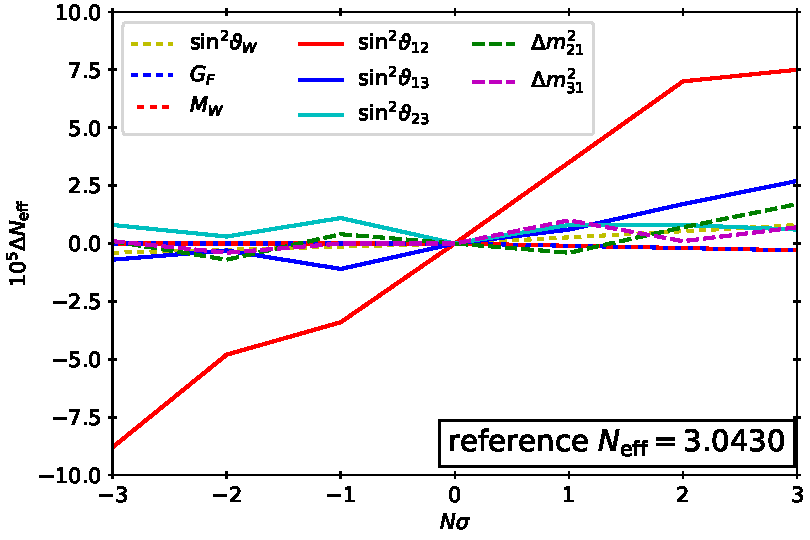
\includegraphics[width=0.49\textwidth]{plots/combined}
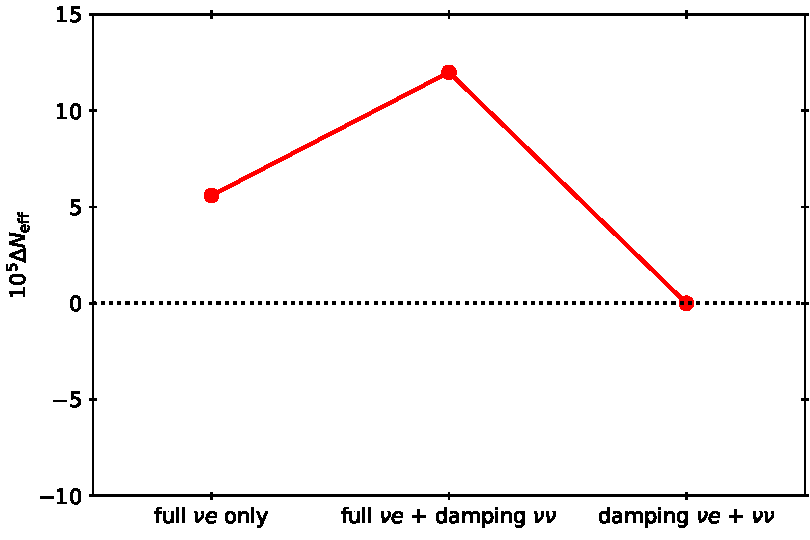
\includegraphics[width=0.49\textwidth]{plots/od}
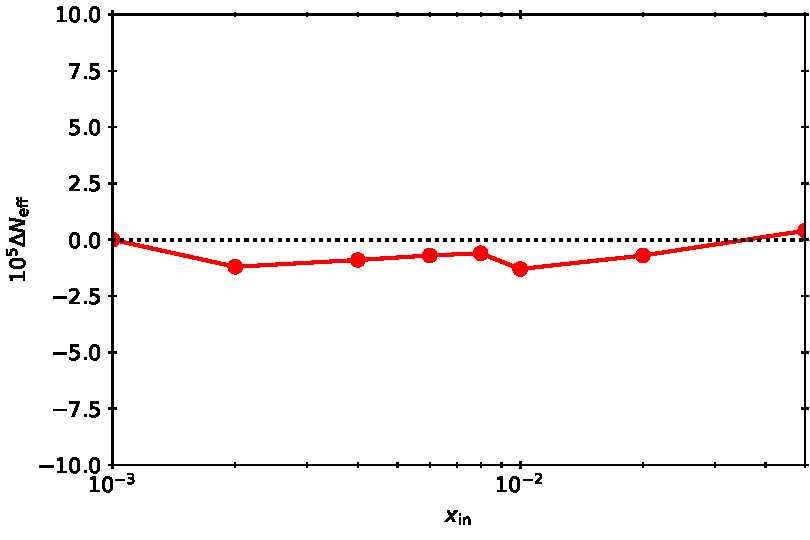
\includegraphics[width=0.49\textwidth]{plots/xin}
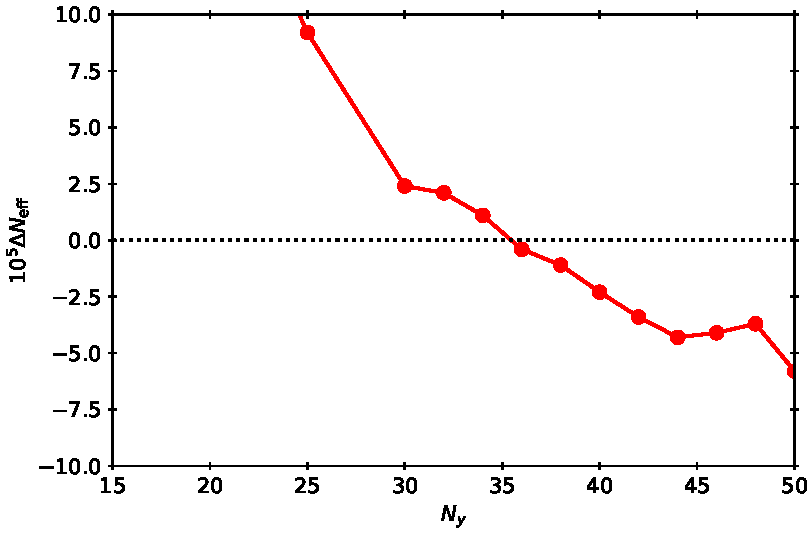
\includegraphics[width=0.49\textwidth]{plots/ny}
\caption{
\label{fig:precision}
Absolute variations of \Neff\ as a function of the physical parameters (upper left)
or of some crucial numerical settings:
the different contributions to the off-diagonal terms of the collision integrals (upper right),
the initial value $x_{\rm in}$ (lower left),
the number of nodes in the $y$ grid (lower right).
}
\end{figure}



\acknowledgments
We thank J.J.~Bennett and G.~Buldgen for helping spotting
some issue in the treatment of finite temperature corrections
and for support in implementing the higher order correction terms.

This software is part of a project that has received funding from the European Union's Horizon 2020 research and innovation programme, under the Marie Sk{\l}odowska-Curie grant agreement No 796941.


\bibliographystyle{JHEP}
\bibliography{main}


\end{document}
